%!TEX root = ../../super_main.tex
\section{Providing Sensor Data}
\label{sec:providing_sensor_data}

To support this structure of the sensor output, we have designed an abstraction over the different sensors available. This abstraction is designed for concurrent collection of samples we want the application for the participants to be able to gather information from multiple sources at the same time, meaning that the system is able to, for instance, collect data regarding the motion and location of the participant simultaneously. This is done in order to make sure that the gathered data is obtained according to the desired temporality of the customer, i.e. the time constraints of the campaign.
\\\\
Problems arose when enforcing temporality of snapshots due to the event oriented nature of sensors in Android. Sensor events will trigger whenever a value is updated. This effectively means that it is impossible to know when these events will trigger. We want to guarantee that measurements can be made with a specific frequency independent on what is supported by the sensor, i.e. measurements can be made more often than what some sensors provide, but also more rarely.    

\begin{figure}[!htbp]
    \centering
    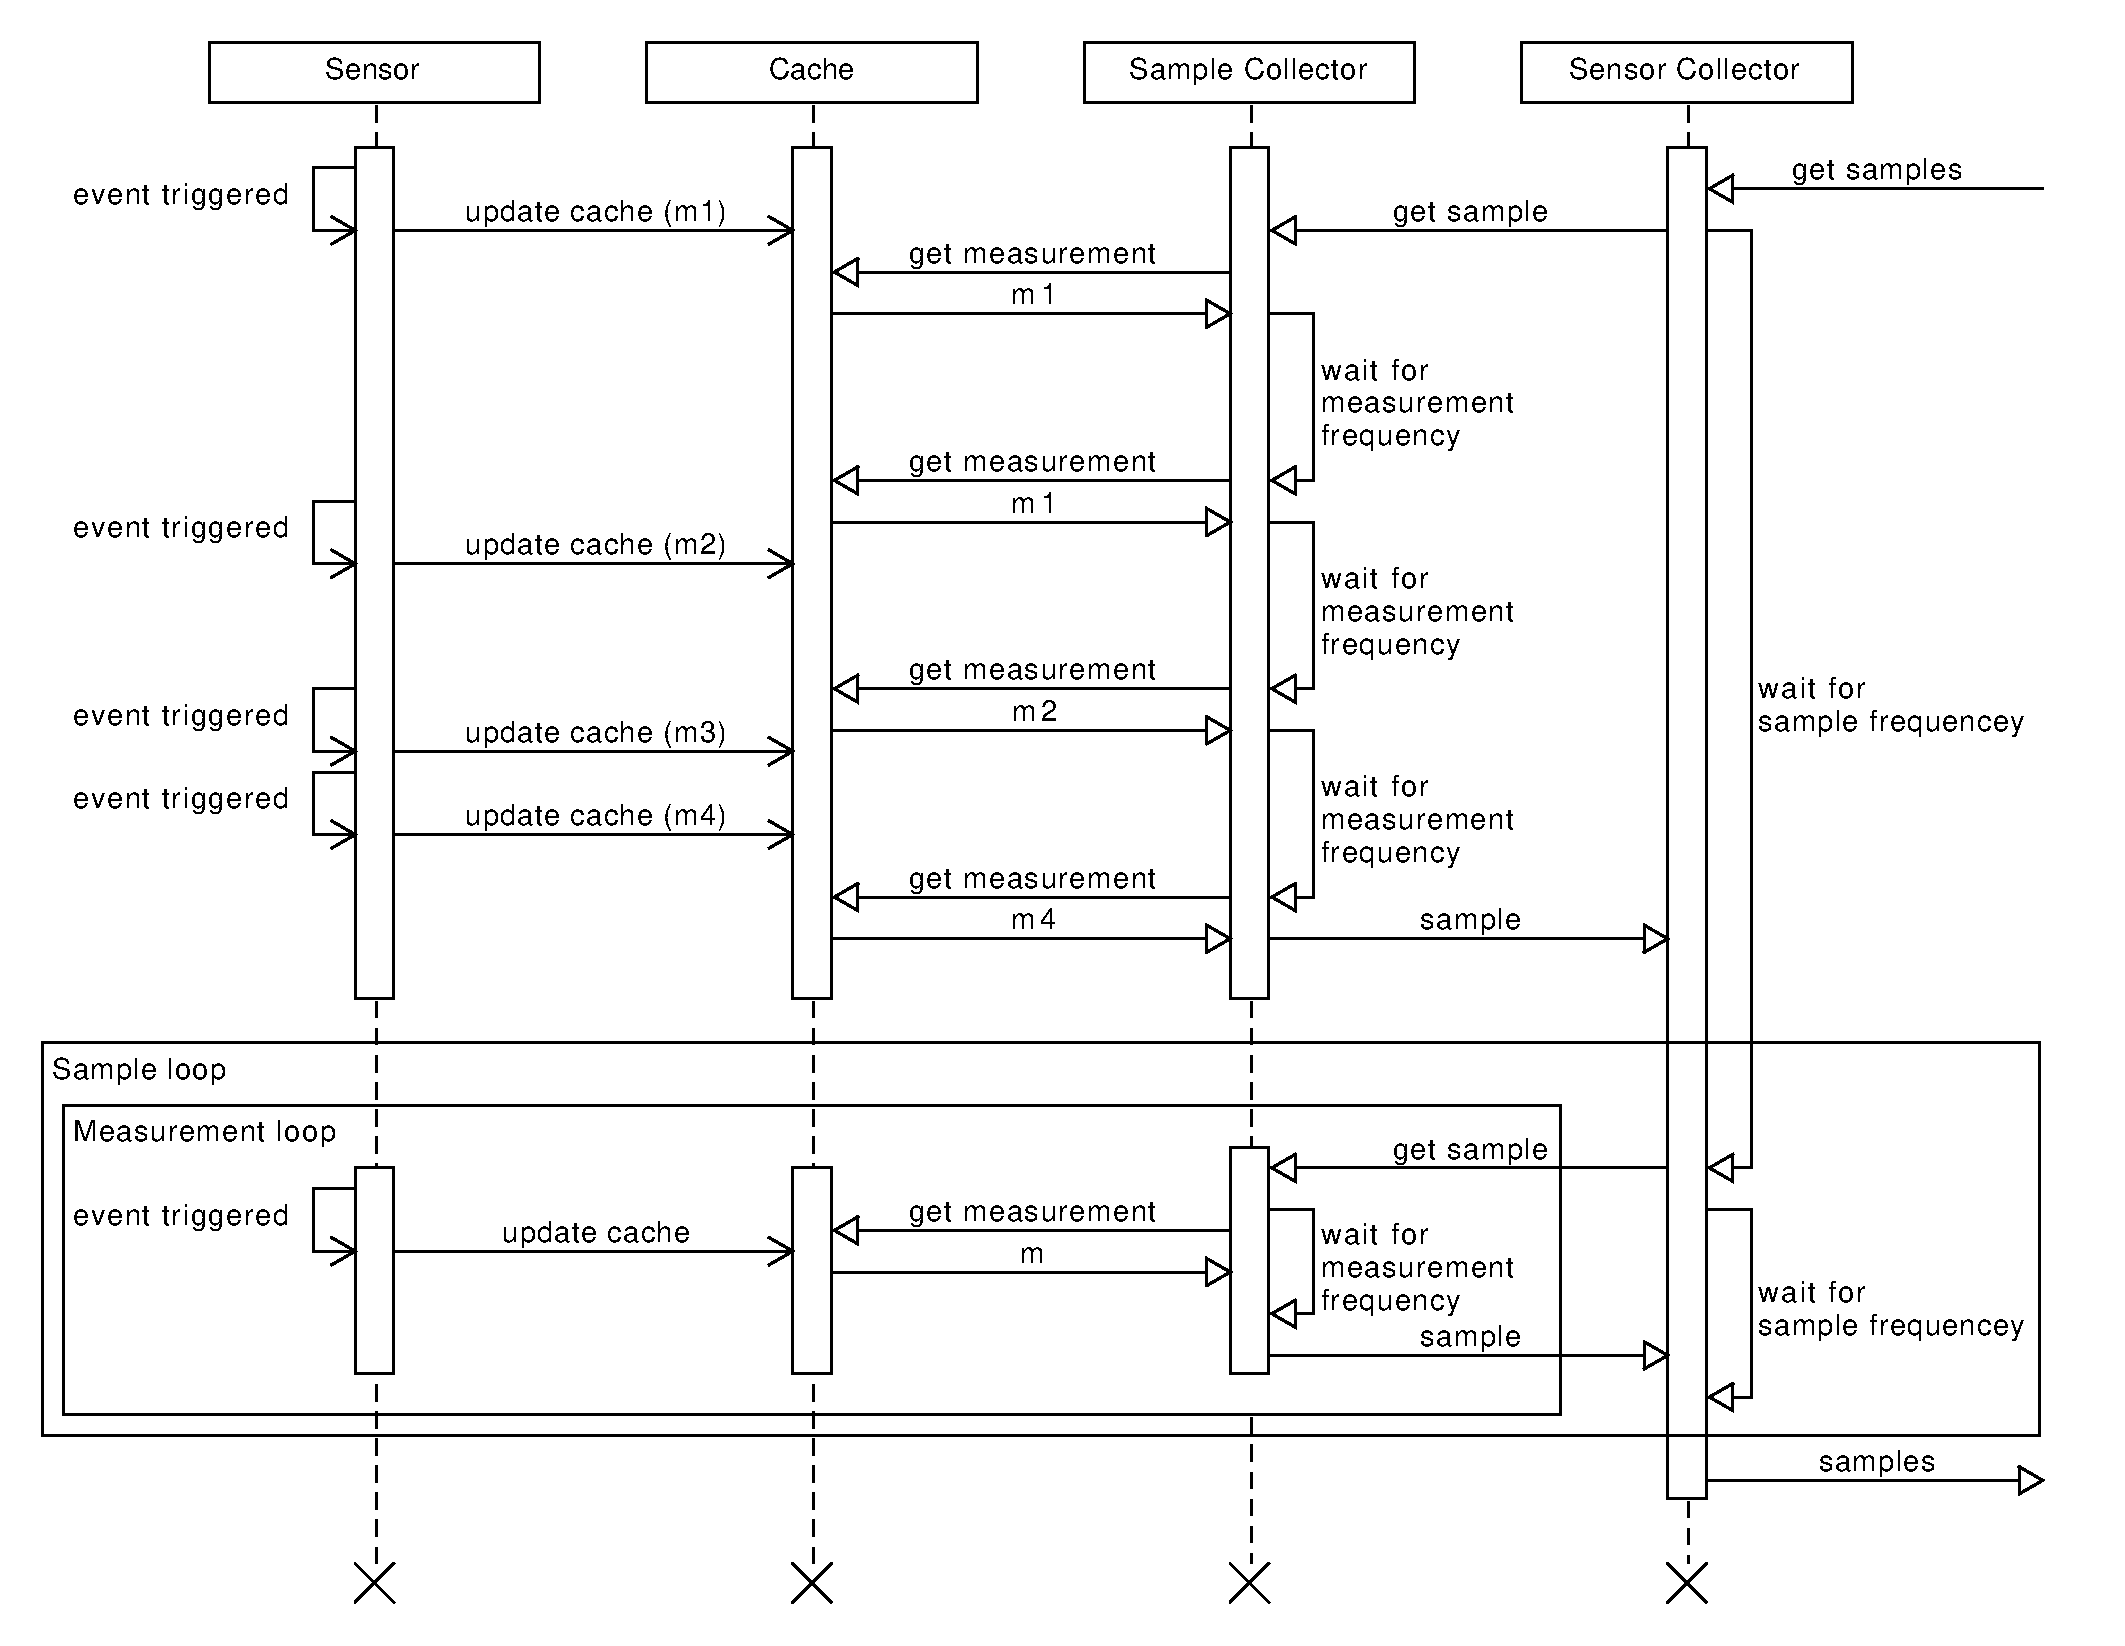
\includegraphics[width=\textwidth]{backgroundsensorservice/cached_values}
    \caption{Snapshot creation based on cache to ensure desired temporality.}
    \label{fig:cached_values}
\end{figure}
\FloatBarrier

\subsection{Implementation}
We have implemented an abstract class called \mono{SensorProvider}, which can be specialized for each type of sensor available. The common interface for these sensor providers is implemented by the following methods:

\begin{itemize}
	\item \mono{abstract boolean isSensorAvailable();}
	\item \mono{abstract Sample retrieveSampleForDuration(long, long);}
	\item \mono{Future<List<Sample>{}> retrieveSamplesForDuration(long, long, long, long);}
\end{itemize}

The abstract \mono{isSensorAvailable()} method allows the subclasses of \mono{SensorProvider} a way of specifically checking if the device has that sensor available. This might for example be useful in order to determine which campaigns should be available to which participants at some point, or detecting if a wearable device has been disconnected. \mono{retrieveSampleForDuration()} is a method that every subclass has to implement, which specifies how a sample is created for this specific sensor. The \mono{retrieveSamplesForDuration()} method is implemented on the \mono{SensorProvider} class, i.e. not abstract like the other two methods, and is the method that makes all the different providers work asynchronously. The method returns a \mono{Future<List<Sample>{}>}. A future, in Android, is the result of an asynchronous computation. The result from a future can be retrieved by calling the \mono{get()} method on the future object, which is a blocking call. Android then provides different methods to check whether or not the computation is completed, in progress, and so on. The method works by submitting a \mono{Callable} to a thread pool, which will eventually return a list of samples, i.e. the future. This callable contains a \mono{TimerTask}, which is a task that is repeated a certain amount of times, that in return calls the \mono{retrieveSampleForDuration()} method. In that way, we have a \mono{Callable} which at some point returns the desired amount of samples. 
\\\\
The \mono{retrieveSampleForDuration()} method has, in all the subclasses of \mono{SensorProvider}, been implemented by using a native method called \mono{onSensorChanged()}. As the name implies, this event is triggered whenever a sensor changes its state. This is a potential issue, since not all sensors provide continuous data, and not all sensors will change in the time limit that is allowed between two measurements (see \figref{fig:sample_temporality}). A potential solution to this is to always store the previous state, and if the event is not triggered within the alloted time, simply use the cached value. 
\\\\
Another potential issue with this implementation is the desire for asynchronism, which we implemented by using \mono{future} objects. Since we cannot know for certain when different asynchronous calls are finished, it might become difficult to create a snapshot and send it to the database.

% \lstinputlisting[
%    style = java,
%    caption = {Property similarity on a component.},
%    label = {lst:attribute_difference},
%]{content/implementation/annotation/attribute_difference.java}